\documentclass[a4paper,12pt]{scrartcl}
\usepackage[ngerman]{babel}
\usepackage[utf8]{inputenc}
\usepackage[verbose]{placeins}
\usepackage{lmodern}
\usepackage{amssymb}
\usepackage{graphicx}
\usepackage{amsmath}
\usepackage{multicol}
\usepackage{enumerate}
\usepackage{verbatim}

\usepackage{float}
%\usepackage{epstopdf}
\usepackage{longtable}
\usepackage{epsfig}
 \usepackage{placeins}
\usepackage{scrpage2}\pagestyle{scrheadings}
\title{Visualisierung der Abläufe des Parallelisierten PDE-Solvers}
\author{Johannes Timm \and Guannan Hu}
\date{\today}
% \chead{\titleinfo}
% \ohead{\today}
% \setheadsepline{1pt}
% \setcounter{secnumdepth}{0}
% \newcommand{\qed}{\quad \square}

\begin{document}
\maketitle
\notag

\section{Visualisierung der Implementierung des Gauss-Seidel und Jacobi Iterationsverfahrens}
\subsection{Konfiguration}
Für alle Tests wurden 20 Iterationen und ein Abbruch nach Iterationen gewählt. Damit einzelne Iterationsschritte erkennbar werden wurden 1000 Interlines gewählt. Um die Konfiguration der Knoten  ordnungsgemäß abzuwickeln wurden die Jobscripte aus de vorherigen Aufgabe angepasst.
\subsection{Jacobi}
\subsubsection{2 Knoten 3 Prozesse}

\begin{figure}[hr!]
 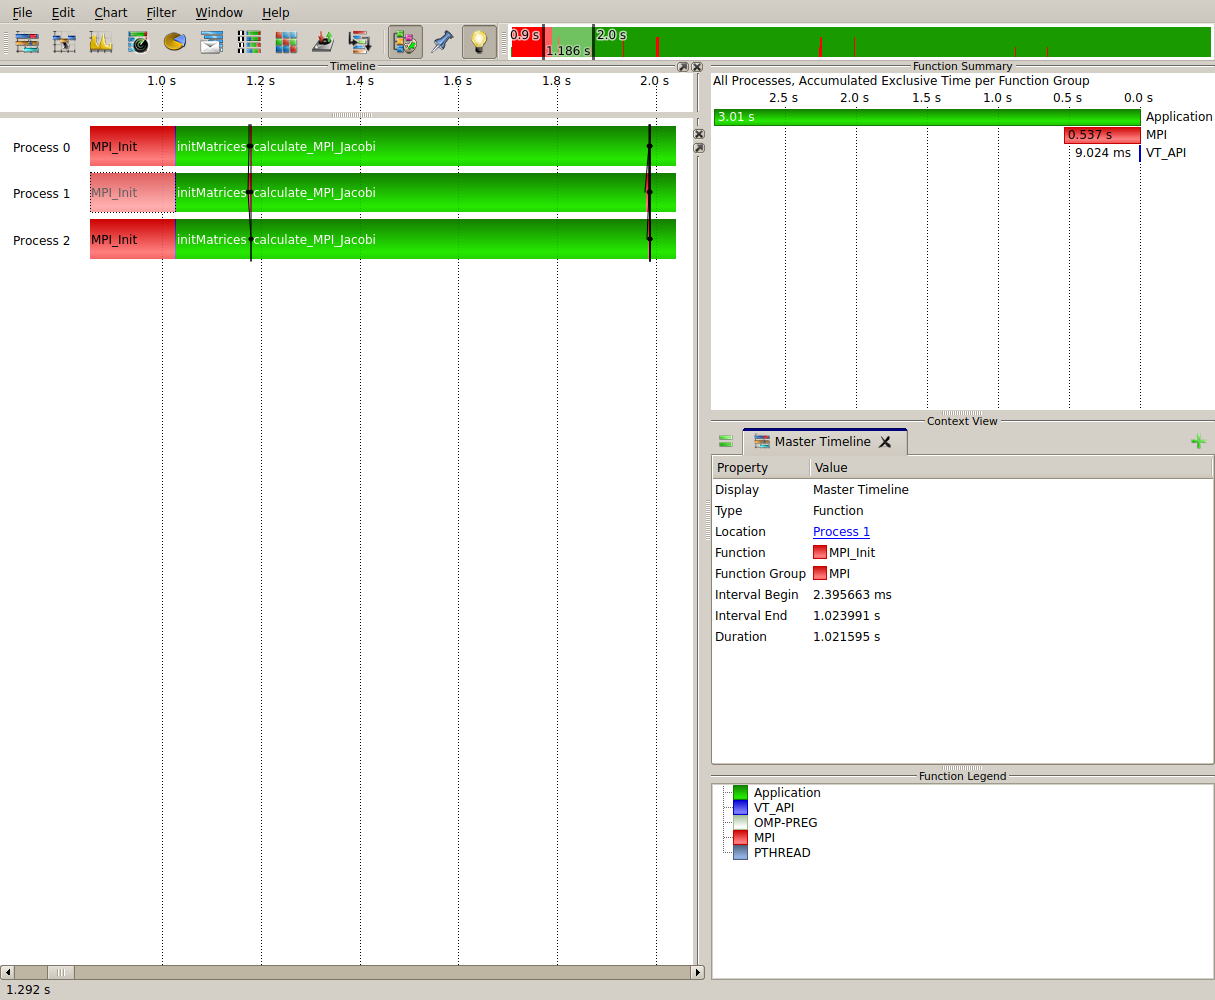
\includegraphics[scale=0.45]{./3_2_JA/Start.png}
 \caption{Der Beginn des Jacobi-Verfahrens bei 3 Prozessen}
\end{figure}
Die Initialisierung der Berechnung nimmt etwa 1s in Anspruch. Das Verteilen der Matrix geht dafür wesentlich schneller. Alle Prozesse sind dank einer Barrier so gut synchronisiert, dass die Kommunikation quasi senkrecht zur Zeitachse verläuft.
\FloatBarrier
\begin{figure}[hr!]
 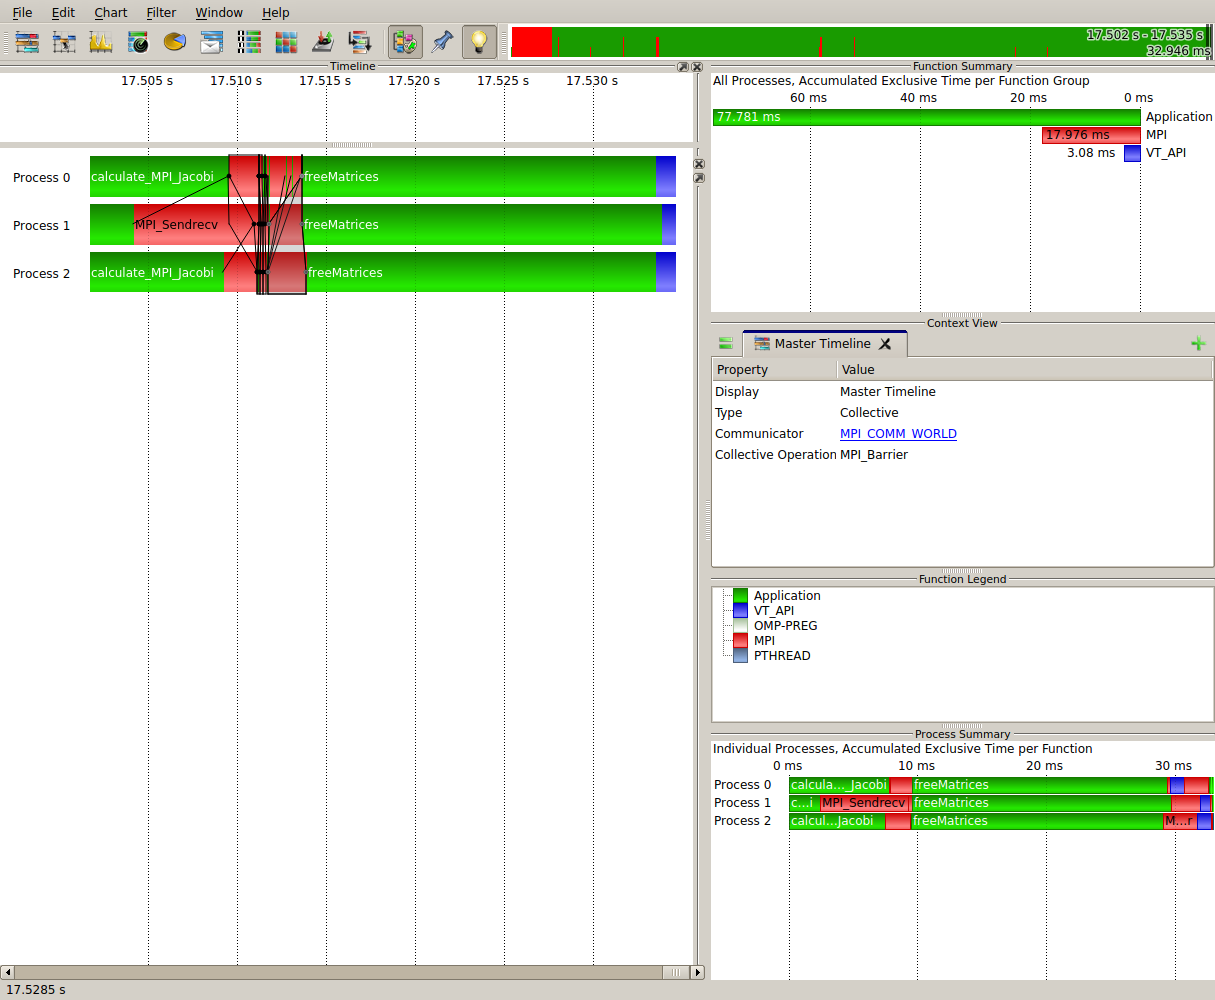
\includegraphics[scale=0.45]{./3_2_JA/End.png}
 \caption{Das Ende des Jacobi-Verfahrens bei 3 Prozessen}
\end{figure}
In dieser Vergrößerung der Beendigung erkennt man einen gewissen Unterschied in der Laufzeit der einzelnen Prozesse. Nach dem letzten Austausch Daten. Wird das Ergebnis von Prozess 0 eingesammelt. Dies passiert so schnell, dass die einzelne Kommunikation hier nur schwer sichtbar ist. Das Freigeben des Speichers dauert jedenfalls wesentlich länger.
\FloatBarrier
\begin{figure}[hr!]
 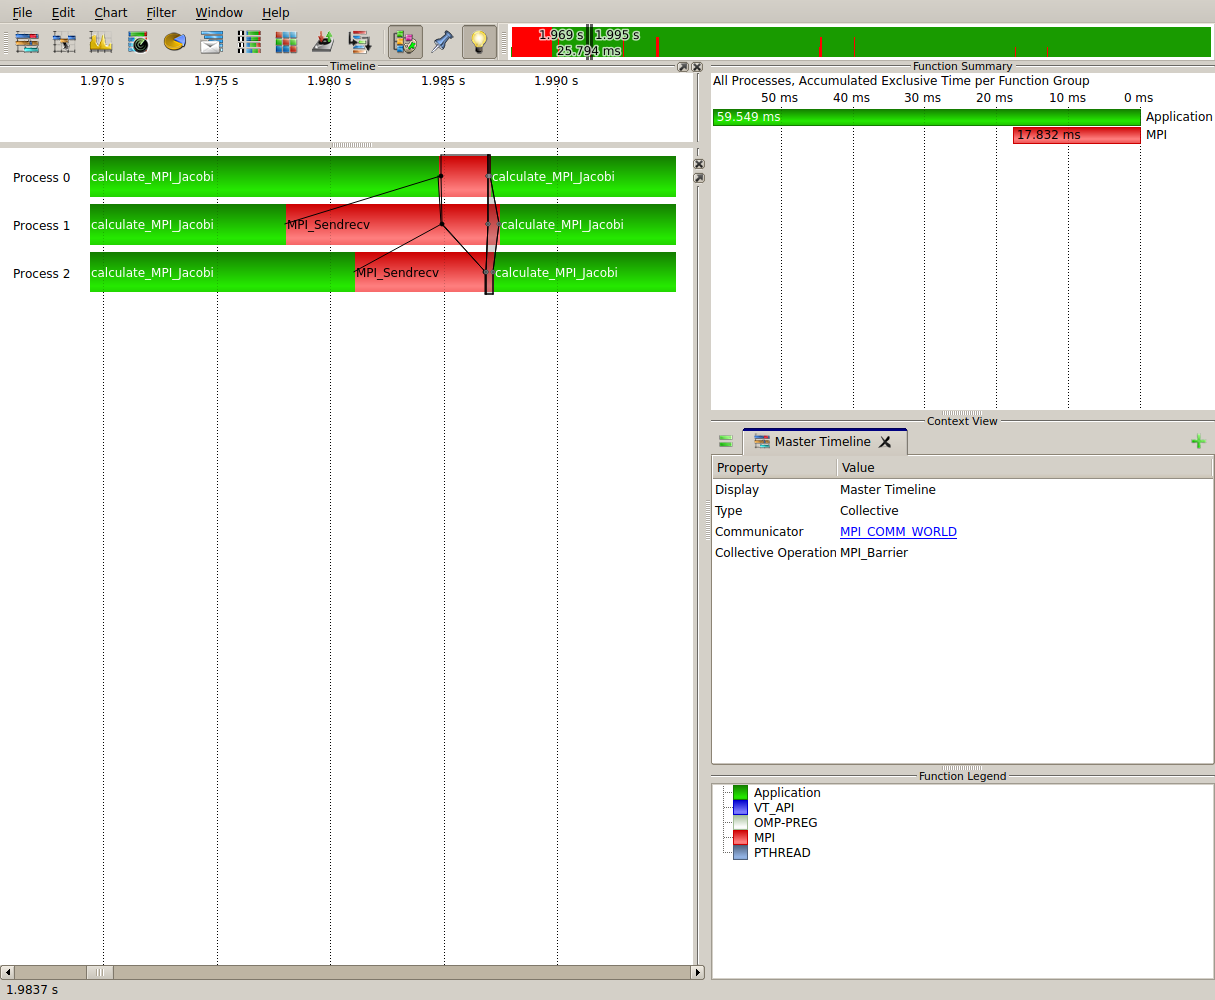
\includegraphics[scale=0.45]{./3_2_JA/Syncronize.png}
 \caption{Die Synchronisation am Ende eines Iterationsschrittes des Jacobi-Verfahrens bei 3 Prozessen}
\end{figure}
Man kann in diesem Bild erkennen, dass nicht alle Prozesse die gleiche Zeit benötigen, um ihrer Iteration zu beenden, durch die Verwendung eines blockierenden SendRecv und anschließendem Allreduce beginnen alle Prozesse zum nahezu gleichen Zeitpunkt mit der nächsten Iteration. Die ungleiche Laufzeit wurde somit ausgeglichen.
\FloatBarrier
\FloatBarrier
\subsubsection{4 Knoten 5 Prozesse}

\begin{figure}[hr!]
 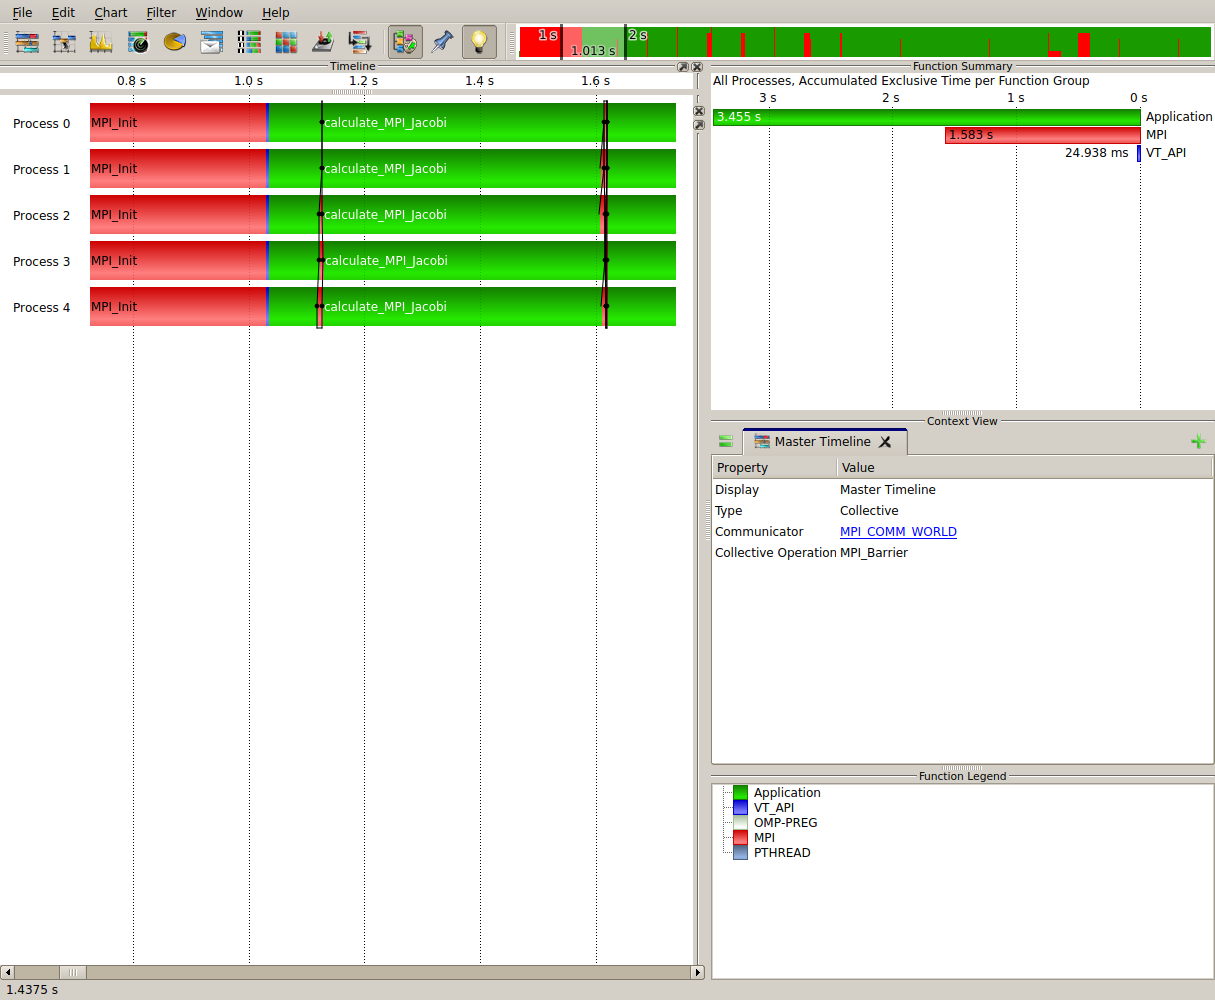
\includegraphics[scale=0.45]{./5_4_JA/Start.png}
 \caption{Der Beginn des Jacobi-Verfahrens bei 5 Prozessen}
\end{figure}
Hier gilt die Beobachtung, dass sich das Laufzeitverhalten zwischen 3 und 5 Prozessen kaum geändert hat. Laufzeitunterschiede zwischen den einzelnen Prozessen treten hingegen etwas öfter und sichtbarer auf. Ein eindeutiger Auslöser für diese Laufzeitschwankungen kann so direkt nicht ausgemacht werden. Die Menge an Knoten ist jedoch  durch die Erhöhung der Latenz zwischen den Nachrichten ein Faktor. 
\FloatBarrier
\begin{figure}[hr!]
 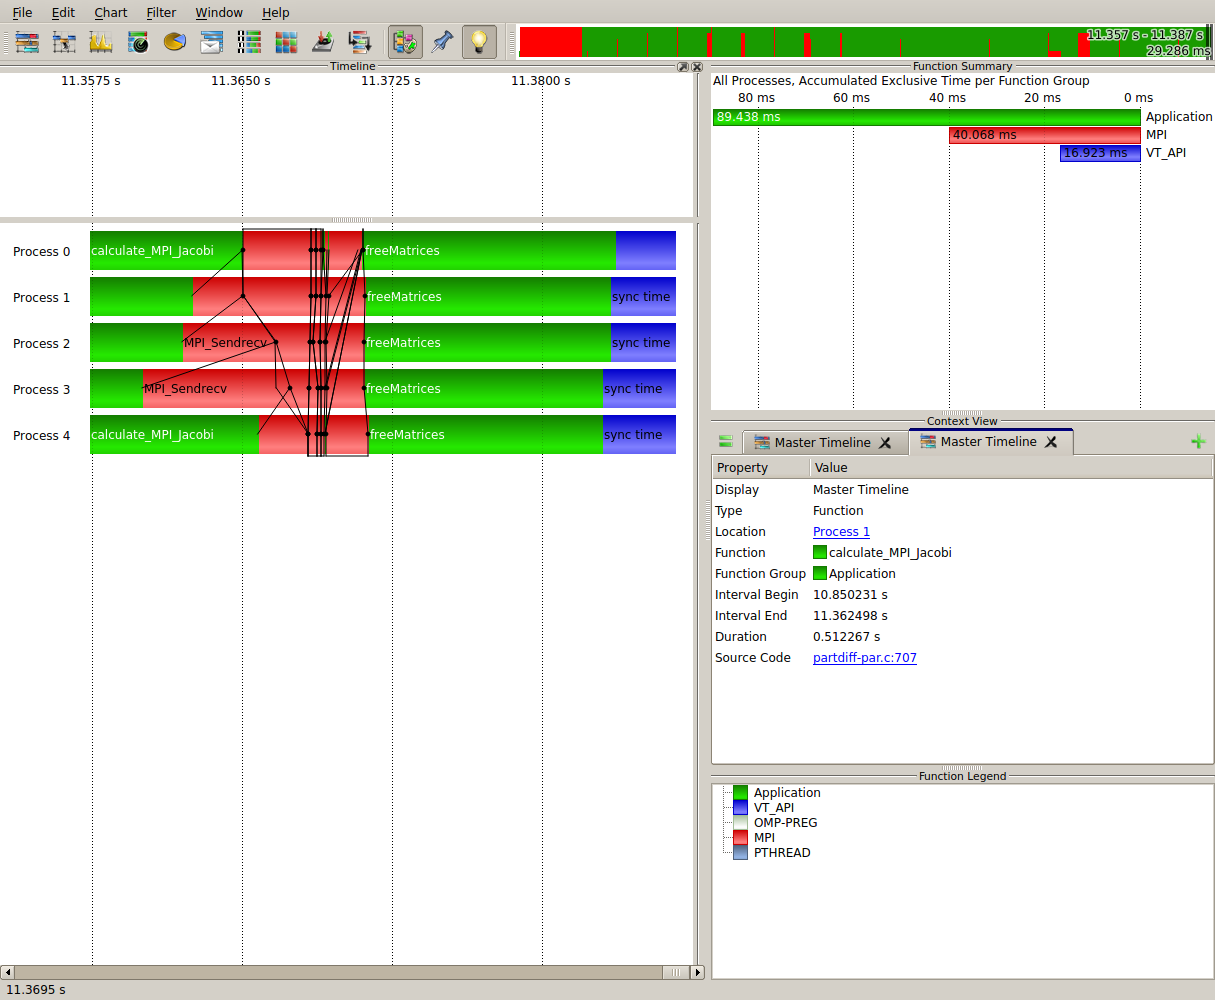
\includegraphics[scale=0.45]{./5_4_JA/End.png}
 \caption{Das Ende des Jacobi-Verfahrens bei 5 Prozessen}
\end{figure}
Auch für die Beendigung der Berechnung gilt obige Beobachtung. Die Prozesse warten eine unterschiedlich lange Zeit auf Ihre Kommunikation. Die Ausgabe ist auch hier so schnell, dass man sie quasi nicht beobachten kann. 
\FloatBarrier
\begin{figure}[hr!]
 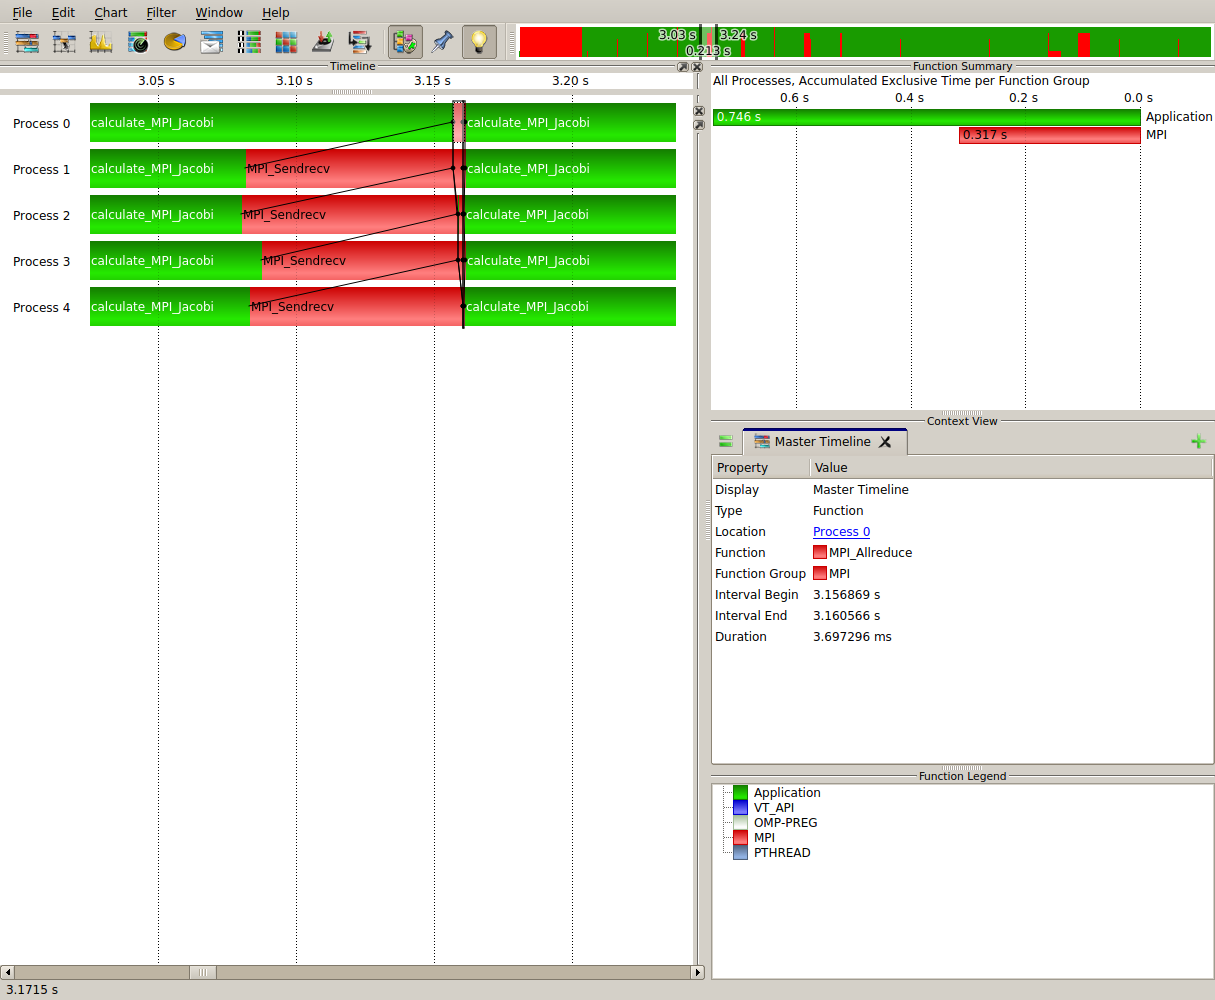
\includegraphics[scale=0.45]{./5_4_JA/Syncronize.png}
 \caption{Die Synchronisation am Ende eines Iterationsschrittes des Jacobi-Verfahrens bei 5 Prozessen}
\end{figure}
Bei der Synchronisation zwischen den Prozessen zeigt sich in dieser Grafik, dass der Prozess 0 etwas mehr rechnet, als die anderen Prozesse. Die Begründung für dieses Verhalten ist durch die Sonderbehandlung des ersten Prozesses im Programmcode gegeben. Die Prozesse sind nach der Kommunikation wieder synchron.
\newpage
\FloatBarrier
\FloatBarrier
\subsection{Gauss-Seidel}
\subsubsection{2 Knoten 3 Prozesse}

\begin{figure}[hr!]
 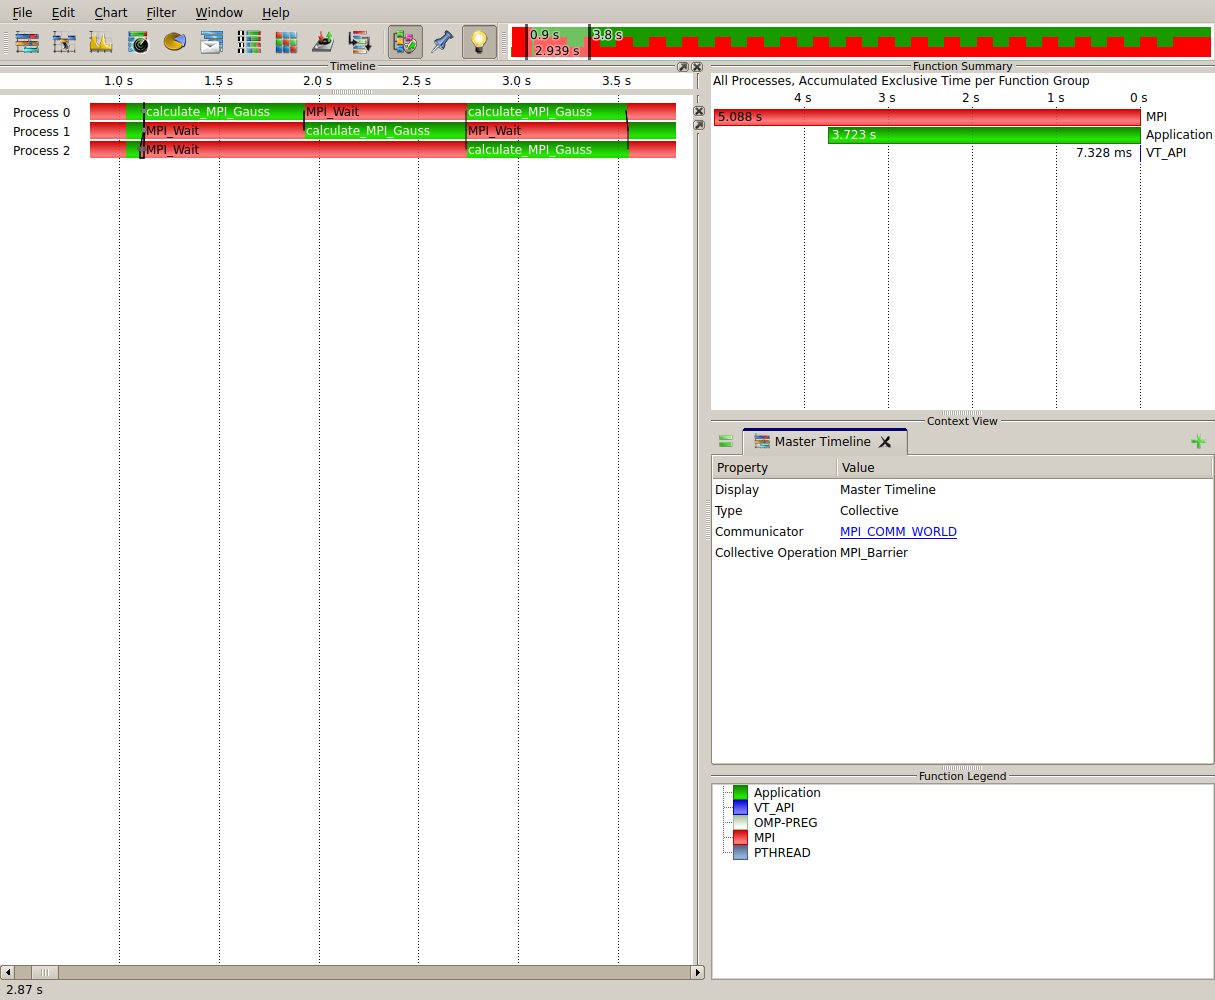
\includegraphics[scale=0.45]{./3_2_GS/Start.png}
 \caption{Der Beginn des Gauss-Seidel-Verfahren bei 3 Prozessen}
\end{figure}
Man kann in diesem Screenshot sehr gut erkennen, dass sich wie gewünscht eine Pipeline aufbaut. Die Initialisierung von MPI dauert auch hier etwa 1 Sekunde. Die Initialisierung der Matrix ist vergleichsweise schnell. Es zeigt sich jedoch bereits hier der bedeutende Performance Bug. Die Tatsache, dass der Prozesse 0 direkt nach seiner Berechnung erst einmal Wartet, bedeutet, dass die Programmlogik hier einen Fehler hat. Wo dieses Wait im Programmcode steckt war leider nicht herauszubekommen, da mehrere davon verwendet werden. Jedenfalls sorgt dieses Verhalten zu einer Reduktion der Geschwindigkeit um Faktor 2. Zudem ist das Verhalten nicht identisch mit dem Verhalten, wie es ursprünglich designt war. 
\FloatBarrier
\begin{figure}[hr!]
 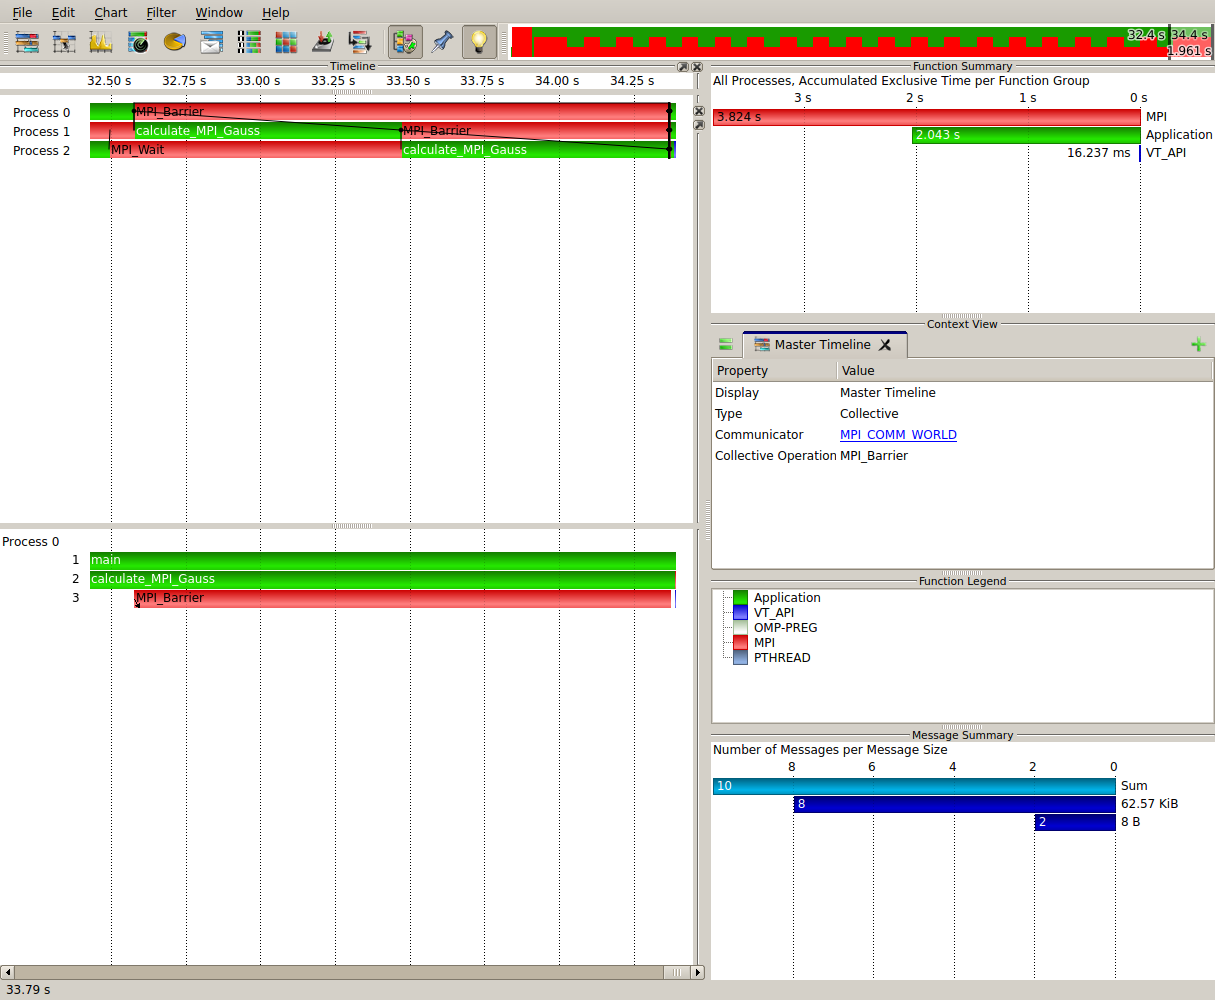
\includegraphics[scale=0.45]{./3_2_GS/End.png}
 \caption{Das Ende der Pipeline des Gauss-Seidel-Verfahren bei 3 Prozessen}
\end{figure}
Das Auslaufen der Pipeline dauert fast genauso lange, wie das Aufbauen. Die letzte Berechnung jedes Prozesses dauert einen Tick länger als in den normalen Iterationen, da etwas zusätzliche Programmlogik ausgeführt wird. Die Barrier dient hier dazu sicherzustellen, dass alle Prozesse in der selben Iteration abbrechen. Die Ausgabe des Programms erfolgt so schnell, dass dies die Laufzeit des Programms nur unwesentlich erhöht.
\FloatBarrier
\begin{figure}[hr!]
 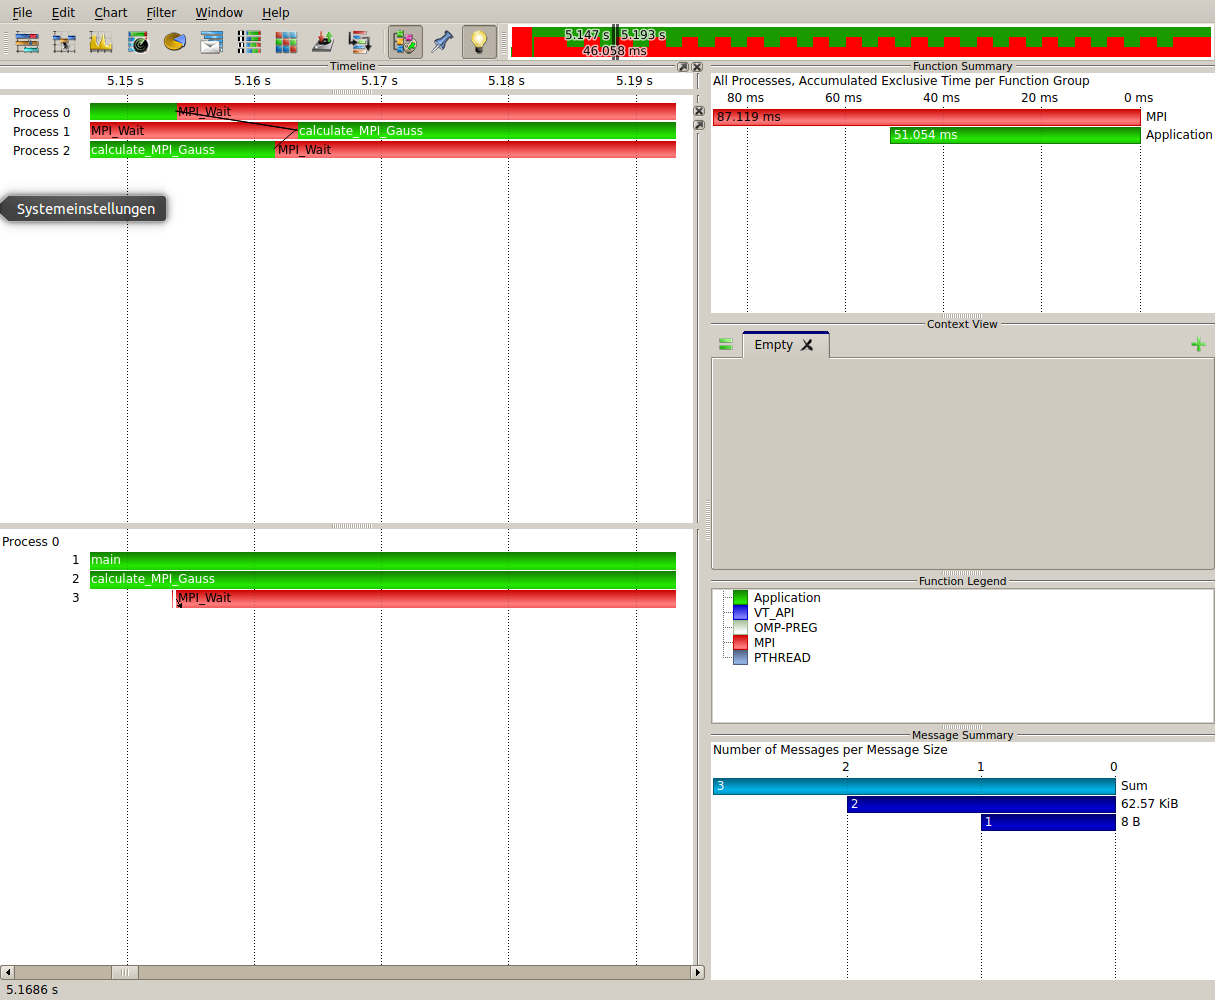
\includegraphics[scale=0.45]{./3_2_GS/Syncronize.png}
 \caption{Die Synchronisation am Ende eines Iterationsschrittes des Gauss-Seidel-Verfahren bei 3 Prozessen}
\end{figure}
In der Synchronisationsphase erkennt man, dass sich nur die benachbarten Prozesse durch die Kommunikation synchronisieren. Eine explizite Synchronisierung findet hier nicht statt. Da keine Kollektive Operation wie Barrier oder Allreduce durchgeführt wird.  
\FloatBarrier
\subsubsection{4 Knoten 5 Prozesse}

\begin{figure}[hr!]
 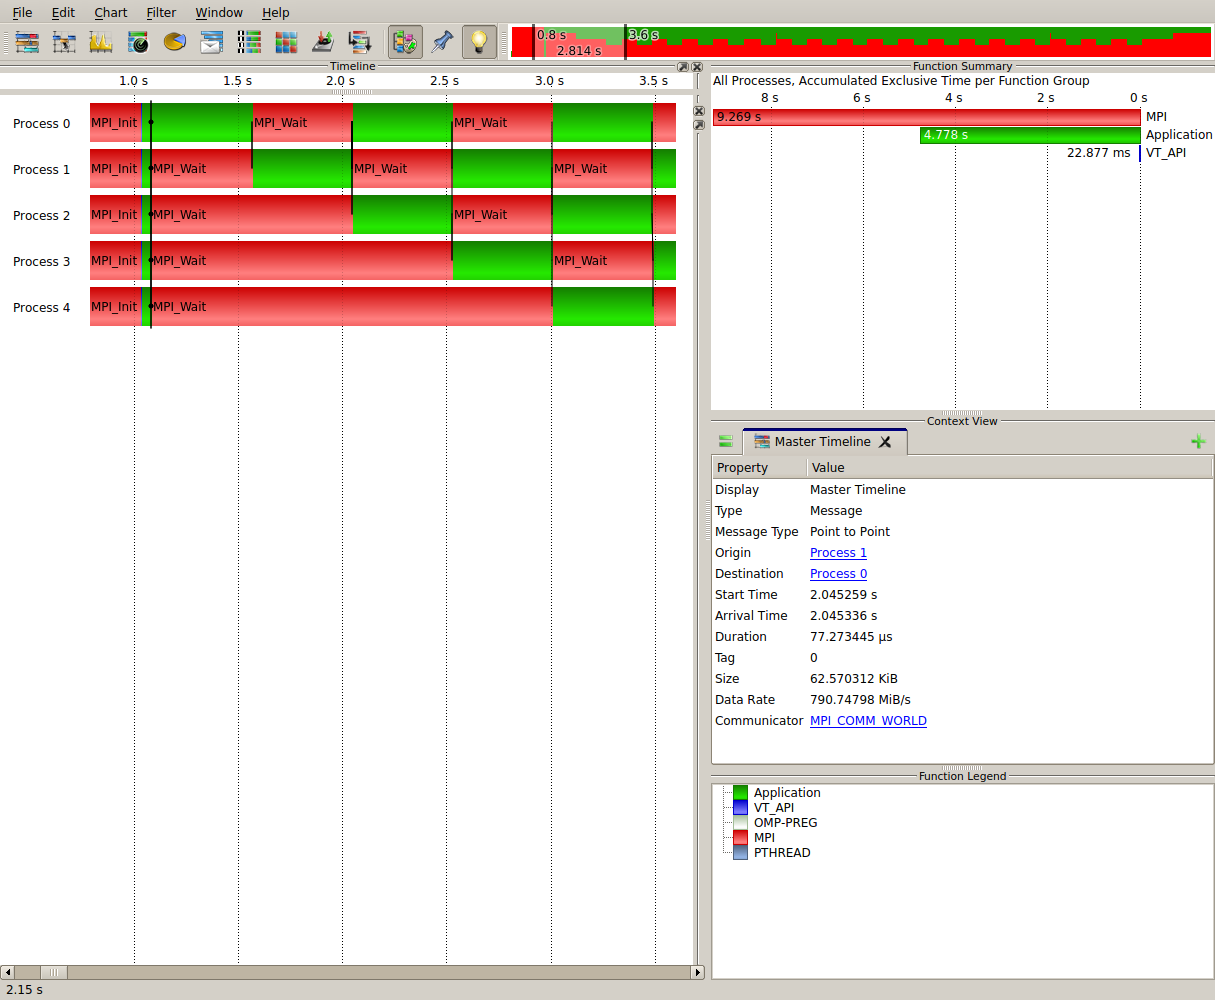
\includegraphics[scale=0.45]{./5_4_GS/Start.png}
 \caption{Der Beginn des Gauss-Seidel-Verfahren bei 5 Prozessen}
\end{figure}
Die Beobachtung ist hier die gleiche, wie im Fall mit 3 Prozessen. der Aufbau des Schachbrettmusters ist jedoch besser erkennbar.  
\FloatBarrier
\begin{figure}[hr!]
 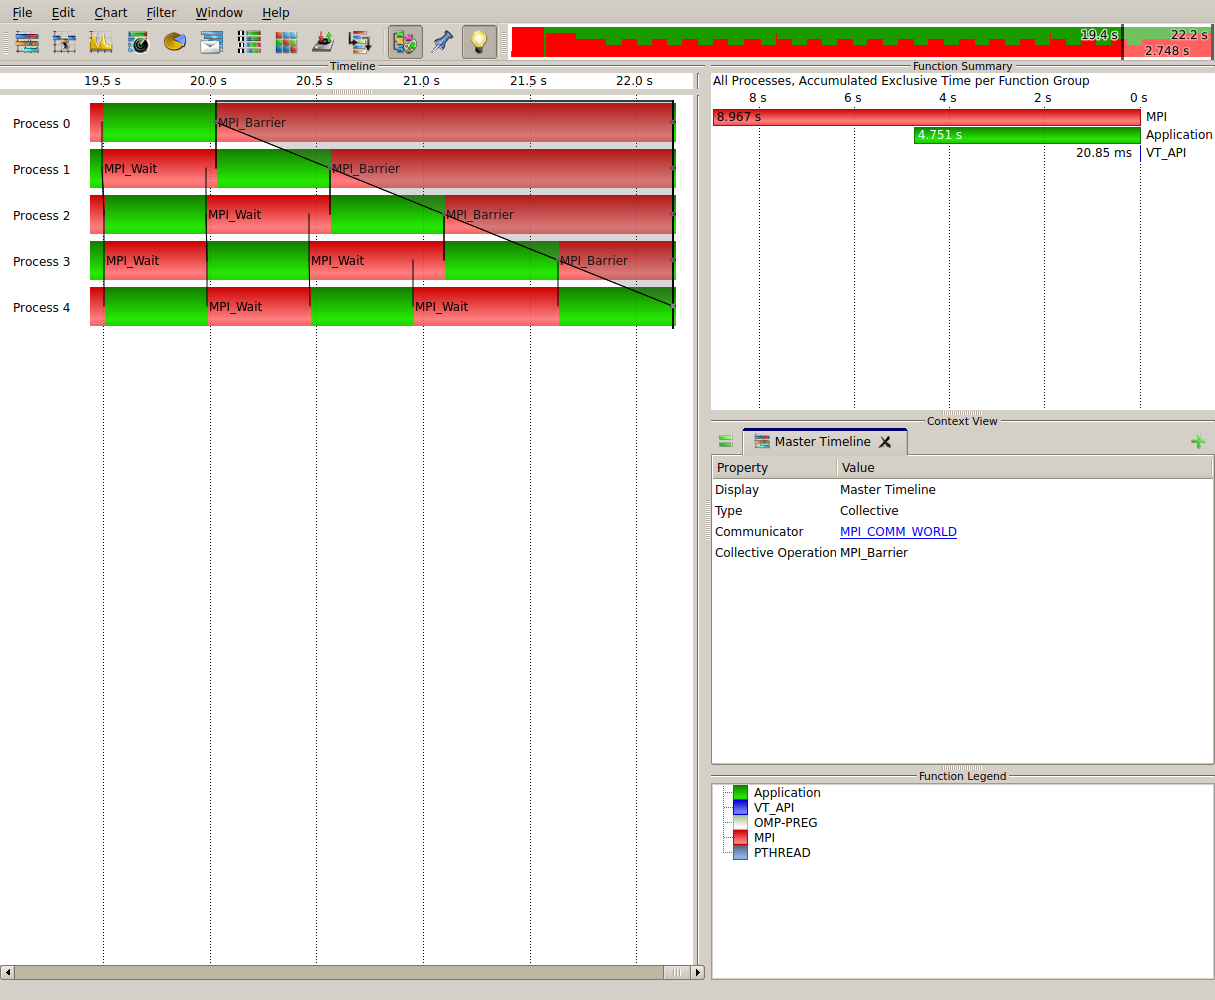
\includegraphics[scale=0.45]{./5_4_GS/End.png}
 \caption{Das Ende der Pipeline des Gauss-Seidel-Verfahren bei 5 Prozessen}
\end{figure}
Die Laufzeitunterschiede zwischen einer normalen Iteration und der letzten Iteration bei allen Prozessen sind hier gut zu erkennen. Die Ausgabe und das Aufräumen sind hier nicht mehr erkennbar, der vertikale grüne Strich am rechten Rand zeigt die Ausgabe und den einzigen kollektiven Austausch der Genauigkeit.
\FloatBarrier
\begin{figure}[hr!]
 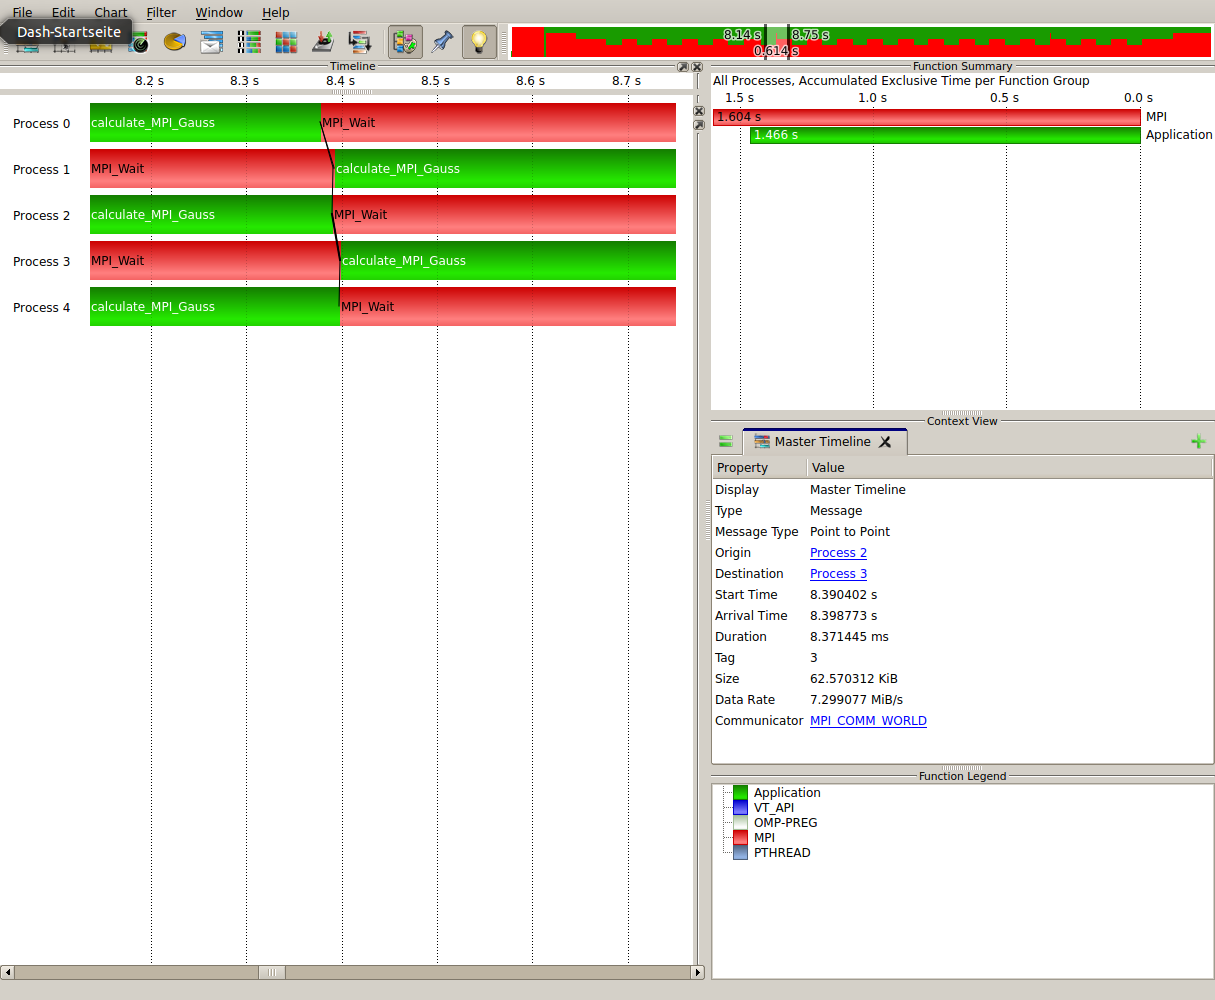
\includegraphics[scale=0.45]{./5_4_GS/Syncronize.png}
 \caption{Die Synchronisation am Ende eines Iterationsschrittes des Gauss-Seidel-Verfahren bei 5 Prozessen}
\end{figure}
Die Synchronisation mit den jeweiligen Nachbarn funktioniert. Das Vorhandensein des Schachbrettmusters ist jedoch hinderlich zur Beurteilung der Güte der Synchronisation in Bezug auf die Vermeidung von Laufzeitverschiebungen.  
\newpage
\FloatBarrier
\FloatBarrier
\subsection{Diskussion}
Das Jacobi Verfahren hat in diesen Konfigurationen, die hier Visualisiert wurden kaum Probleme performant zu arbeiten Es kommt beim Jacobi-Verfahren nie vor, dass Desynchronisationen länger als einen Iterationsschritt andauern. Die ist eine Folge aus der Benutzung der Blockierenden Kommunikation von Allreduce und SendRecv, sodass alle Prozesse am Abschluss eines Iterationsschrittes aufeinander warten. 
Beim Gauss-Seidel-Verfahren ist durch das Pipelineing anfälliger für Desyncronistation, leider ist sie auch wesentlich schwerer zu erkennen. Die Prozesse des Gauss-Seidel-Verfahrens scheinen sich ledoch größtenteils sehr gut dynamisch miteinander zu synchronisieren.
Ein Fehler in der Kommunikationsstruktur des Gauss-Seidel-Verfahrens wurde jedoch offenbar, da sich die Berechnung jeweils mit einem Wait gleicher Länge abwechselt. Leider wird aus der Visualisierung nicht offenbar, in welcher Zeile des Programmcodes dieses spezifische Wait aufgerufen wird. Dies ergibt ein Schachbrettmuster. Dieses führt dazu, dass im Durchschnitt 50\% der Rechenzeit für Warten vergeudet wird. Eine Änderung des Verhaltens der spezifischen Wait -funktion in ein Wait mittels Interrupt würde die Energieeffizienz der Berechnung mit dem Gauss-Seidel-Verfahren erhöhen, ohne dass Änderungen an der Kommunikationsstruktur und ggf. Algorithmus vorzunehmen sind.  
Dies erklärt beim Gauss-Seidel-Verfahren die Differenz in der Ausführungsgeschwindigkeit zwischen einem und zwei Prozessen, da der Overhead des zusätzlichen Prozesses vorhanden ist, jedoch effektiv nur einer Rechnet.
Eine Diskussion der Fälle von 4 und 10 Knoten ist aufgrund der gewonnenen Erkenntnisse beim Gauss-Seidel Verfahren nicht mehr sinnvoll, da das Schachbrettmuster zuerst eliminiert werden muss. 
Beim Jacobi-Verfahren zeigte der Fall von 4 Knoten keine Auffälligkeiten. Eine Untersuchung für 10 Knoten wurde (noch) nicht durchgeführt.
\end{document}